% Journal version — targeted at Language Resources and Evaluation (Springer).
%
% Springer's current template class (sn-jnl.cls) is distributed through
% Springer/Overleaf rather than CTAN. If sn-jnl.cls is present next to this
% file (or the project is opened from Springer's Overleaf template), it is
% used automatically; otherwise a self-contained single-column fallback that
% approximates the Springer layout compiles with a plain TeX Live install so
% the manuscript can always be built and read locally.
%
% Journal requirement honoured here: decimal headings, no more than three
% levels.
\IfFileExists{sn-jnl.cls}{%
  \documentclass[sn-basic]{sn-jnl}%
  \newcommand{\usingsnstyle}{}%
}{%
  \documentclass[11pt]{article}%
  \usepackage[a4paper,top=2.5cm,bottom=2.5cm,left=3cm,right=3cm]{geometry}%
  \usepackage{times}%
  \usepackage[round]{natbib}%
  \usepackage{setspace}%
  \onehalfspacing%
  \usepackage[hidelinks]{hyperref}%
}

\usepackage[T1]{fontenc}
\usepackage[utf8]{inputenc}
\usepackage{microtype}
\usepackage{booktabs}
\usepackage{graphicx}
\usepackage{url}
\emergencystretch=3em

\newcommand{\corpusname}{Saudi Legal Corpus for AI}

\title{The Saudi Legal Corpus for AI: An Auditable,
Official-Source-Grounded, Article-Level Corpus of Saudi Arabian
Legislation}

\ifdefined\usingsnstyle
  \author*[1]{\fnm{Abdullah} \sur{Almohammedi}}\email{abdullah.m.almohammedi@gmail.com}
  \affil[1]{\orgname{Independent Researcher}}
\else
  \author{Abdullah Almohammedi \\
    Independent Researcher \\
    \texttt{abdullah.m.almohammedi@gmail.com} \\
    ORCID: \href{https://orcid.org/0009-0001-0832-0995}{0009-0001-0832-0995}}
  \date{}
\fi

\begin{document}

\maketitle

\begin{abstract}
Legal natural language processing has advanced rapidly for English and
several European languages, but Arabic --- and Saudi Arabian law in
particular --- remains critically under-resourced: to our knowledge, no
openly documented, machine-readable, article-level corpus of Saudi
legislation has previously been described. We present the \corpusname, a
corpus of 290 legislative instruments (201 statutory laws, 64 statutory
regulations, 24 implementing regulations, and one set of procedural rules)
covering the Kingdom of Saudi Arabia's principal legislation, structured
into 15{,}689 article-level records ($\sim$1.2 million Arabic tokens) in a
unified, retrieval-ready index spanning twelve legal domains. The corpus
rests on three design commitments that distinguish it from web-scraped
legal collections: official-source grounding, in which every track records
its issuing authority and official source and every record carries its own
provenance label (251 distinct labels) under a four-tier source-verification
taxonomy; auditability, enforced by 376 read-only, idempotent validators and
fully deterministic derived layers; and the governing-text principle, under
which the official Arabic text governs and all other language layers are
explicitly non-authoritative. Beyond the text, the corpus ships analytical
layers that are, to our knowledge, the first of their kind for Saudi law: a
statutory citation graph (3{,}607 references, 585 of them between distinct
instruments), a hand-classified supersession graph (102 edges), a glossary
of 1{,}920 statutorily defined terms with 3{,}318 definitions, an
embedding-ready chunking layer (16{,}304 chunks), and a manually confirmed
retrieval benchmark of 519 gold queries. On that benchmark the corpus's
metadata-based lexical searcher reaches 93.3\% top-1 accuracy against 90.4\%
for a standard BM25 baseline, with the gap concentrated on definitional
queries (90.9\% versus 74.5\%), quantifying the value of the engineered
retrieval metadata while leaving informative headroom for neural Arabic
legal retrieval. We describe the construction methodology in full, report
statistics that are reproducible from the archived release, and discuss
intended uses, limitations, and the legal and ethical boundaries of
releasing structured national legislation for artificial-intelligence
research.
\end{abstract}

\ifdefined\usingsnstyle
\keywords{Legal NLP, Arabic language resources, Saudi Arabia, Legislative
corpus, Information retrieval, Data provenance}
\else
\vspace{1em}\noindent\textbf{Keywords:} Legal NLP $\cdot$ Arabic language
resources $\cdot$ Saudi Arabia $\cdot$ Legislative corpus $\cdot$
Information retrieval $\cdot$ Data provenance
\vspace{1em}
\fi

\section{Introduction}
\label{sec:intro}

Large language models are increasingly consulted for legal questions, and
retrieval-augmented generation (RAG) over authoritative legal text is the
standard mitigation for hallucinated law. That mitigation is only available
where authoritative legal text exists in machine-readable, retrieval-ready
form. For the law of the Kingdom of Saudi Arabia --- a G20 economy that has
recently undergone a major codification wave, including a new Civil
Transactions Law (721 articles), a new Companies Law (281 articles), a new
Evidence Law, and a new Personal Status Law --- no such resource has, to our
knowledge, been publicly documented. Saudi legislation is published
officially in the \emph{Umm Al-Qura} gazette and on government portals as
human-readable pages and PDF documents; it is not distributed as structured,
article-level, provenance-annotated data.

This paper presents the \corpusname, which closes that gap. The corpus
structures the principal body of Saudi legislation into canonical
article-level JSON with explicit provenance, wraps it in deterministic
validation, and derives from it a unified retrieval index, a chunking layer,
citation and supersession graphs, a glossary of statutory definitions, and a
manually confirmed retrieval benchmark.

Our contributions are fourfold. First, the corpus itself: 290 legislative
instruments and 15{,}689 article-level records, approximately 1.2 million
Arabic tokens, spanning twelve legal domains from commercial and civil law
through criminal procedure, labour, taxation, technology regulation, and the
institutional statutes of major authorities (Section~\ref{sec:contents}).
Second, a methodology for auditable legal corpora: official-source grounding
with per-record provenance labels, a four-tier source-verification taxonomy,
a freshness manifest that documents known staleness risks instead of hiding
them, and 376 read-only idempotent validators (Section~\ref{sec:design}). We
argue that this methodology is a reusable template for legal corpora in any
jurisdiction that lacks a machine-readable official gazette. Third, derived
analytical layers unavailable elsewhere for Saudi law: a citation graph, a
hand-classified supersession graph, and a statutory-definition glossary
(Section~\ref{sec:layers}). Fourth, a retrieval evaluation resource: 519
manually confirmed gold queries with two deterministic baselines reported
per query category (Section~\ref{sec:retrieval}).

Throughout, the corpus maintains a strict legal-status boundary. It is not
an official government publication, it contains no official translation, and
the official Arabic text governs; English and Chinese layers are
non-authoritative references. We return to these boundaries in
Section~\ref{sec:ethics}.

\section{Related work}
\label{sec:related}

\subsection{Legal corpora and benchmarks}

Large legal text collections and benchmarks now exist for English and
several European jurisdictions: the Pile of Law
\citep{henderson2022pileoflaw}, MultiLegalPile
\citep{niklaus2024multilegalpile}, LexGLUE \citep{chalkidis2022lexglue},
LEXTREME \citep{niklaus2023lextreme}, CUAD \citep{hendrycks2021cuad}, and
LegalBench \citep{guha2023legalbench}. These resources are dominated by
English and European languages; none includes Saudi legislation, and Arabic
is at most marginally represented.

Table~\ref{tab:comparison} positions the \corpusname\ against these
resources. It is smaller by raw volume --- deliberately so, since it is a
structured statute corpus rather than a pretraining dump --- and it is the
only one that is simultaneously article-level, Arabic-governing, and
provenance-annotated at the level of the individual record.

\begin{table}[t]
\centering
\footnotesize
\begin{tabular}{@{}lllll@{}}
\toprule
\textbf{Resource} & \textbf{Type} & \textbf{Languages} & \textbf{Unit} & \textbf{Provenance} \\
\midrule
Pile of Law & pretraining & English & document & no \\
MultiLegalPile & pretraining & 24 (no Arabic) & document & per source \\
LexGLUE & benchmark & English & task example & no \\
LEXTREME & benchmark & 24 (no Arabic) & task example & no \\
LegalBench & benchmark & English & task example & no \\
\midrule
\corpusname & corpus $+$ eval & Arabic (gov.); EN/ZH ref. & article & per record \\
\bottomrule
\end{tabular}
\caption{Positioning against existing legal corpora and benchmarks.
``gov.'' denotes the governing layer; ``ref.'' denotes non-authoritative
reference layers (English and Chinese currently cover one law). Per-record
provenance here means 251 distinct source-status labels organized under a
four-tier verification taxonomy.}
\label{tab:comparison}
\end{table}

\subsection{Arabic legal NLP}

Arabic NLP infrastructure has matured considerably
\citep[e.g.,][]{antoun2020arabert, obeid2020camel}, and domain-specific
models such as AraLegal-BERT \citep{alqurishi2022aralegal} have been trained
on proprietary Arabic legal text. Openly documented \emph{data resources}
for Arabic law --- in particular structured, provenance-annotated statute
corpora --- nevertheless remain scarce. To our knowledge, no prior published
resource provides article-level, machine-readable coverage of Saudi
legislation with documented official-source provenance.

\subsection{Legal document standards and citation networks}

Standards such as Akoma Ntoso \citep{palmirani2011akoma} and the European
Legislation Identifier define structural markup for legislation. Our
canonical JSON is deliberately simpler --- flat article-level records with
rich retrieval metadata --- but is convertible to such standards. A separate
literature applies network science to legal citation structure
\citep{fowler2007network, katz2014complexity, coupette2021measuring}; the
citation and supersession graphs we release (Section~\ref{sec:layers}) are,
to our knowledge, the first machine-readable inputs enabling that line of
work for Saudi, and more broadly Gulf, legislation.

\section{Source material: the Saudi legislative landscape}
\label{sec:sources}

Saudi legislation is enacted primarily by royal decree
(\emph{ni\d{z}\={a}m}, conventionally rendered ``law'' or ``system'') and
elaborated by implementing regulations issued by ministers or authorities,
alongside procedural rules, ministerial decisions, and official model forms.
The authoritative publication channel is the official gazette \emph{Umm
Al-Qura}; consolidated texts are additionally published on official portals,
principally the Bureau of Experts at the Council of Ministers
(\url{laws.boe.gov.sa}) and the Ministry of Justice legal portal
(\url{laws.moj.gov.sa}), as well as on the sites of issuing ministries and
authorities.

Three unit terms recur in this paper and in the data at different
granularities, and we fix them here. A \textbf{track} is the registry's unit
of management: one onboarded instrument-layer bundle with its own sources,
validators, and reports (291 tracks, of which 290 correspond to legislative
instruments and one is a repository-level audit artifact). An
\textbf{instrument} (\texttt{law\_id}) is one enacted law, regulation, or
rule set as identified in the unified index; 283 appear there. A
\textbf{corpus} (\texttt{corpus} key) is a subject-matter grouping that
typically joins a law with its implementing regulation and annexes --- the
\texttt{labor} corpus, for example, spans eight components --- of which
there are 199.

Each track records its Arabic and English display names, issuing authority,
official source URL or URLs, publication dates in both the Hijri and
Gregorian calendars where available, language layers, record counts, and
validator targets, in a central machine-readable registry (registry version
3.0).

\section{Corpus design and methodology}
\label{sec:design}

\subsection{Design principles}

The corpus is built around four commitments.

\emph{The official Arabic text governs.} Every record carries the official
Arabic text verbatim (\texttt{text\_ar}); no summarization, normalization,
or editorial rewriting is applied to the governing text. All non-Arabic
layers are explicitly flagged as non-authoritative.

\emph{Provenance is per-record and honest.} Every record in the unified
index carries a \texttt{text\_status} provenance label describing exactly how
its text was obtained and verified --- for example, a cross-check between
the Ministry of Justice portal application programming interface and the
published official PDF. There are 251 distinct provenance labels,
deliberately fine-grained rather than collapsed into a small ordinal scale,
because collapsing provenance destroys auditability. Where a primary portal
was found stale at build time, such as an amendment the portal had not yet
incorporated, that fact is documented rather than silently patched: the
freshness manifest flags 16 of 291 tracks as carrying a known
source-staleness risk.

\emph{Validation is read-only, deterministic, and idempotent.} The
repository ships 376 validator targets, of 476 total build targets, that
check schema conformance, record counts, hashes, layer boundaries, and
cross-layer consistency without mutating any data. Derived-layer generators
make no network calls and consult no wall-clock time, so every layer is
exactly reproducible from the committed sources.

\emph{Derived layers are additive projections.} The unified index, chunking
layer, graphs, glossary, verification tiers, and freshness manifest are all
read-only projections over the canonical track files. None of them alters
legal text, and each records what it was generated from.

\subsection{Source verification tiers}

Because Saudi Arabia has no machine-readable official gazette, source
quality varies by track and must be represented rather than assumed. Every
track is assigned to one of four verification tiers
(Table~\ref{tab:tiers}). The taxonomy allows downstream users to filter by
evidential strength: a production RAG deployment may restrict itself to
Tiers~1 and~2, while a coverage-oriented study may accept all four with the
recorded caveats attached.

\begin{table}[t]
\centering
\small
\begin{tabular}{lr}
\toprule
\textbf{Tier} & \textbf{Tracks} \\
\midrule
1 --- primary sources, multiple, in agreement & 127 \\
2 --- primary source cross-verified against secondary & 88 \\
3 --- secondary sources only, multiple, in agreement & 39 \\
4 --- single source, or mixed confidence & 37 \\
\midrule
\textbf{Total} & \textbf{291} \\
\bottomrule
\end{tabular}
\caption{Source-verification tier assignments across all tracks.}
\label{tab:tiers}
\end{table}

\subsection{Record schema}

The atomic unit is the article-level record (Figure~\ref{fig:record}). In
the unified retrieval index each record carries a stable
\texttt{record\_id}; corpus and track identifiers (\texttt{corpus},
\texttt{law\_id}, \texttt{law\_component}); the official Arabic law title and
the article number; generated retrieval metadata (\texttt{llm\_title\_ar},
\texttt{retrieval\_title\_ar}, \texttt{keywords\_ar},
\texttt{search\_queries\_ar}); the verbatim governing text
(\texttt{text\_ar}); the provenance label (\texttt{text\_status}); and the
source layer file from which it was projected. Records are self-contained: a
single retrieved record carries sufficient context to cite the law, the
component, and the article.

\begin{figure}[t]
\centering
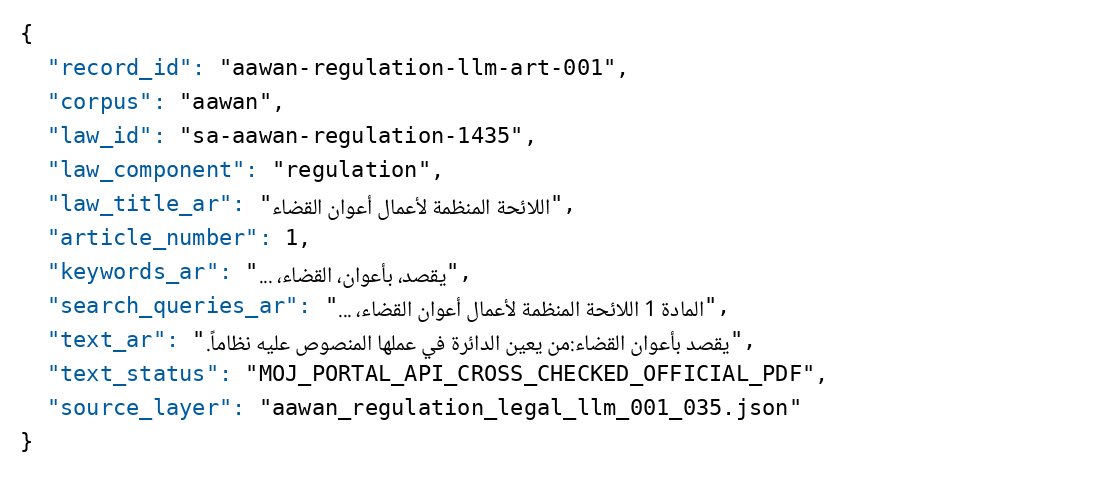
\includegraphics[width=\textwidth]{example_record.png}
\caption{An example unified-index record (Article~1 of the Regulation of
Judicial Assistants' Work, abridged: the keyword and query lists are
truncated). The article text translates as ``Judicial assistants means:
those who assist the circuit in its work as prescribed by law.'' The
\texttt{text\_status} label records that the text was cross-checked between
the Ministry of Justice portal interface and the published official PDF.}
\label{fig:record}
\end{figure}

\subsection{Metadata generation and disclosure of automated assistance}
\label{sec:disclosure}

Resource papers increasingly document not only what a dataset contains but
how each field came to be \citep{bender2018data, gebru2021datasheets}. We
therefore state the generation provenance of each field class explicitly.
The governing Arabic text (\texttt{text\_ar}) is ingested verbatim from the
recorded official sources and is never generated, summarized, or normalized;
validators enforce this by hash and count. The retrieval metadata is
produced mechanically by each track's deterministic generator script ---
keywords by term-frequency extraction from the article's own text, search
queries and retrieval titles by number and title templates --- and not by a
generative model, which is why the metadata-based searcher evaluated in
Section~\ref{sec:retrieval} is deterministic end to end. The non-governing
reference layers, namely the English layers and the internal Chinese layer,
were produced with machine-assisted translation and passed a documented
internal quality-assurance programme; they are explicitly non-official and
non-binding. Repository tooling and documentation were developed with
AI assistance; every data-bearing layer that this tooling produces is
regenerable deterministically and checked by read-only validators.

\section{Corpus contents and statistics}
\label{sec:contents}

All figures reported in this section are computed by a read-only statistics
script released with the corpus and are reproducible from the archived
release cited in the data-availability statement.

\subsection{Composition by instrument type}

\begin{table}[t]
\centering
\small
\begin{tabular}{lr}
\toprule
\textbf{Corpus family} & \textbf{Tracks} \\
\midrule
Statutory laws & 201 \\
Statutory regulations & 64 \\
Implementing regulations & 24 \\
Procedural rules & 1 \\
\midrule
\textbf{Legislative instruments} & \textbf{290} \\
Repository-level audit artifact & 1 \\
\midrule
\textbf{Total registry tracks} & \textbf{291} \\
\bottomrule
\end{tabular}
\caption{Composition of the corpus by instrument type. The audit artifact
is a quality-assurance record, not legislation, and carries no legal text.}
\label{tab:families}
\end{table}

Table~\ref{tab:families} gives the composition by instrument type. The
registry counts 16{,}753 records in total: 15{,}858 primary Arabic governing
records, 614 reference records in the English layers, and 281 internal
reference records in the Chinese layer for the Companies Law. The unified
retrieval index projects 15{,}689 of the primary governing records; the
remaining 169 belong to a separate implementing-regulations intake track
family that is registry-counted but served through its own layer files.

\subsection{The unified retrieval index}

\begin{table}[t]
\centering
\small
\begin{tabular}{lr}
\toprule
\textbf{Measure} & \textbf{Value} \\
\midrule
Article-level records & 15{,}689 \\
Distinct legislative instruments & 283 \\
Distinct subject-matter corpora & 199 \\
Arabic tokens (whitespace-delimited) & 1{,}206{,}097 \\
Characters & 7{,}123{,}487 \\
Distinct provenance labels & 251 \\
\bottomrule
\end{tabular}
\caption{The unified retrieval index at a glance.}
\label{tab:index}
\end{table}

Table~\ref{tab:index} summarizes the unified index and
Table~\ref{tab:components} breaks its records down by component type. The
long tail of component types --- procedural manuals, model contract forms,
recruitment rules, accessibility arrangements --- reflects a deliberate
decision to ingest the official annexes that accompany major laws rather
than the statute text alone, since those annexes carry operative content
that practitioners consult directly.

\begin{table}[t]
\centering
\small
\begin{tabular}{lr}
\toprule
\textbf{Component} & \textbf{Records} \\
\midrule
Law articles & 8{,}384 \\
Regulation articles & 4{,}655 \\
Implementing-regulation articles & 2{,}113 \\
Procedural manuals & 135 \\
Model contract forms & 102 \\
Model work regulation & 75 \\
Recruitment services rules & 72 \\
Other rules, guides, mechanisms, annexes & 153 \\
\midrule
\textbf{Total} & \textbf{15{,}689} \\
\bottomrule
\end{tabular}
\caption{Unified-index records by component type.}
\label{tab:components}
\end{table}

\subsection{Coverage by legal domain}

The registry records no domain field, since domain membership is not a
property of a Saudi legislative instrument. To convey coverage breadth to
the reader we therefore applied an author-assigned grouping, implemented as
explicit ordered keyword rules over track and corpus identifiers and
released with the corpus so that it can be inspected and revised. Every
track and every indexed record falls into exactly one of the twelve domains
of Table~\ref{tab:domains}; nothing is left unclassified, and the grouping
should be read as an organizing device for this paper rather than as a legal
taxonomy.

\begin{table}[t]
\centering
\small
\begin{tabular}{lrr}
\toprule
\textbf{Legal domain} & \textbf{Instruments} & \textbf{Records} \\
\midrule
Courts, procedure and enforcement & 42 & 3{,}377 \\
Commercial and corporate & 32 & 1{,}605 \\
Financial and capital markets & 30 & 1{,}272 \\
Health, environment and safety & 29 & 946 \\
Civil, personal status and property & 28 & 1{,}681 \\
Energy, industry and infrastructure & 28 & 1{,}766 \\
Criminal justice, security and civil status & 26 & 1{,}038 \\
Technology, data, telecommunications and IP & 20 & 633 \\
Education, culture, media and civil society & 20 & 963 \\
Labour and social insurance & 16 & 1{,}377 \\
Tax and zakat & 11 & 699 \\
Constitutional and administrative & 8 & 332 \\
\midrule
\textbf{Total} & \textbf{290} & \textbf{15{,}689} \\
\bottomrule
\end{tabular}
\caption{Coverage by legal domain under an author-assigned grouping (see
text). Domain membership is assigned by published, inspectable rules and is
not a property of the legislation itself.}
\label{tab:domains}
\end{table}

Coverage is broadest in adjudication and procedure, which is expected: the
procedural instruments are long (the Sharia Procedure regulation alone
contributes 637 articles) and each is accompanied by implementing rules.
The comparatively small record counts in the technology and constitutional
domains reflect the brevity of those instruments rather than gaps in
coverage; the Personal Data Protection Law, for instance, is a complete
track at 43 articles plus its regulations.

\subsection{Multilingual layers}

The Saudi Companies Law (Royal Decree M/132, 1443H; 281 articles) is the
first track to receive full multilingual treatment: the governing Arabic
layer, a full English layer of 281 records, an English reference layer of
281 records, and an internal Chinese reference layer that passed a
documented four-phase remediation and quality-assurance programme closed by
a repository-level audit. The corpus explicitly does not claim trilingual
alignment or an official translation; the multilingual layers exist to
support cross-lingual access research under the governing-text principle.

\section{Derived analytical layers}
\label{sec:layers}

\subsection{Citation graph}

A deterministic extractor scans all 15{,}689 records for statutory
citations, yielding 3{,}607 references: 3{,}022 within a single instrument
and 585 between distinct instruments. Each reference is emitted with the raw
citation text, source and target identifiers, and a confidence label; 3{,}087
are high-confidence and 520 medium-confidence, with no ambiguous-scope
cases. The 585 inter-instrument edges span 191 distinct source tracks and
316 distinct cited target names. The most frequently cited targets are the
Labour Law with 34 inbound citations, the Companies Law with 30, the
Bankruptcy Law with 19, and the Sharia Procedure Law with 14 --- a
distribution that already suggests which instruments function as structural
hubs of the Saudi legal system. This is, to our knowledge, the first
machine-readable citation network over Saudi legislation, and it directly
enables network-analytic studies of centrality, clustering, and dangling
references to superseded instruments.

\subsection{Supersession graph}

A separate layer records repeal and replacement relationships between
instruments: 102 edges, each classified by hand against the corpus's own
documented text, namely registry notes and official-source metadata, and
never inferred from the relative age of decrees or from topical similarity.
Ambiguous cases, and title collisions that are not repeal relationships, are
kept in dedicated sections rather than forced into the edge set. Combined
with the citation graph, this layer supports temporal legal dynamics
research, such as identifying live instruments that still cite repealed
ones.

\subsection{Statutory-definition glossary}

Saudi laws conventionally open with a definitions article. A parser over
these articles yields a corpus-wide glossary of 1{,}920 terms carrying
3{,}318 definitions, extracted from the 214 tracks whose definitions
articles parse cleanly. Because the same term --- ``establishment'' or
``competent authority'', for instance --- is defined independently by many
laws, the glossary is the raw material for studying definitional
fragmentation and terminological consistency across a national legal system.

\subsection{Freshness manifest}

A deterministic, network-free manifest surveys every track's recorded source
URLs, fetch dates, and known discrepancies, and flags 16 tracks as carrying
a documented risk that the primary portal's consolidated text was stale at
build time. A separate live checker, explicitly outside the quality-assurance
gate, can re-probe reachability and drift without compromising the
determinism of the committed layers.

\section{Retrieval index, chunking, and baseline evaluation}
\label{sec:retrieval}

\subsection{Chunking layer}

For embedding pipelines, a chunking layer segments the unified index into
16{,}304 chunks sized in whitespace-delimited words and deliberately not
tied to any particular embedding tokenizer. Of the source records, 15{,}344
fit within a single chunk and 345 long articles are split; each chunk
carries its source record identifier, article number, chunk index, and exact
character offsets into the source text, so that any vector hit remains
traceable to its governing article. No embeddings are computed within the
repository: the layer is pure, traceable segmentation.

\subsection{Gold-query evaluation set}

The retrieval evaluation pack contains 519 Arabic queries, each paired with
a manually confirmed gold article identified by corpus, component, and
article number. Golds were confirmed against the articles' own text or
official structure rather than reverse-engineered from search output, so the
metrics measure the searcher honestly. The queries are categorized: 384
topical, 61 provision-lookup, 55 definitional, and 19 distributed across
smaller categories covering governance, rights, procedure, and deliberately
hard cases.

The queries and golds were authored by a single annotator, the corpus
maintainer, by reading each article's committed text first and writing the
query from its own wording. There is consequently no inter-annotator
agreement to report, and the set inherits an in-vocabulary bias that we
quantify below. Provision-lookup queries such as ``Article~5 of the Labour
Law'' share their surface form with the templated
\texttt{search\_queries\_ar} metadata, so for that category the evaluation
partly measures template matching rather than free-form retrieval. The
per-category breakdown that follows keeps this visible instead of averaging
it away.

\subsection{Baseline results}

We report two deterministic baselines. The \emph{metadata searcher} is the
corpus's own lexical scorer over each record's generated retrieval metadata,
using weighted keyword, title, and query matching with no embeddings and no
learned parameters. \emph{BM25} is standard Okapi BM25 with $k_1 = 1.5$ and
$b = 0.75$ over each record's law title, article title, and verbatim text,
with light Arabic orthographic normalization --- diacritics and tatweel
stripped, and alef, teh-marbuta, and alef-maqsura variants folded --- and
whitespace tokenization, without stemming or a stopword list.
Table~\ref{tab:baseline} reports overall and per-category results; the 19
small-category queries are included in the overall row but not broken out.

\begin{table}[t]
\centering
\small
\begin{tabular}{lrrrr}
\toprule
 & \multicolumn{2}{c}{\textbf{Metadata searcher}} & \multicolumn{2}{c}{\textbf{BM25}} \\
\cmidrule(lr){2-3}\cmidrule(lr){4-5}
\textbf{Query set} & \textbf{Top-1} & \textbf{MRR@5} & \textbf{Top-1} & \textbf{MRR@5} \\
\midrule
All (519) & 93.3 & .956 & 90.4 & .937 \\
Topical (384) & 93.2 & .957 & 92.7 & .956 \\
Provision lookup (61) & 98.4 & .984 & 98.4 & .984 \\
Definitional (55) & 90.9 & .937 & 74.5 & .809 \\
\bottomrule
\end{tabular}
\caption{Top-1 accuracy (per cent) and mean reciprocal rank at rank~5 on the
519-query evaluation set, comparing the corpus's metadata-based searcher
against standard BM25 over titles and verbatim text.}
\label{tab:baseline}
\end{table}

Three observations follow. First, the near-identical provision-lookup scores
confirm the template-matching effect disclosed above: both systems resolve
``Article $n$ of law $X$'' queries almost perfectly, so that category carries
little information about retrieval quality. Second, the gap between the two
systems concentrates precisely where retrieval is hardest. On definitional
queries --- where a query such as ``definition of the sale contract'' shares
few surface tokens with the defining article --- the engineered metadata is
worth 16.4 points of top-1 accuracy over BM25. Third, six queries defeat the
metadata searcher entirely, falling outside the top five; per-query results
for both systems are published, which makes error analysis reproducible.

The remaining headroom, and more importantly robustness to paraphrase and
dialectal variation that the gold queries do not exercise, is precisely the
space in which neural Arabic legal retrievers should be evaluated. We
release the queries, the golds, the per-query results, and both runner
scripts to support that comparison.

\section{Intended uses}
\label{sec:uses}

The corpus is designed to serve five broad uses. As \emph{grounding for
retrieval-augmented Saudi-law assistants}, its per-record provenance and
verification tiers allow deployments to filter by evidential strength rather
than treating all text as equally trustworthy. As a resource for
\emph{Arabic legal NLP research}, it supports retrieval, summarization,
question answering, terminology extraction, and cross-lingual legal access
over a morphologically rich and highly formulaic register of Modern Standard
Arabic. For \emph{computational legal studies}, the released graphs enable
citation-network analysis, studies of definitional consistency, work on the
relationship between laws and their implementing regulations, and analysis
of the temporal dynamics of the recent codification wave. As
\emph{ground truth for factuality benchmarking}, it provides the reference
against which model hallucination on Saudi legal questions can be measured.
Finally, the construction methodology is offered as a \emph{template} for
building auditable legal corpora in other jurisdictions lacking a
machine-readable official gazette.

\section{Limitations}
\label{sec:limitations}

The corpus is not exhaustive. Its 290 instruments cover the principal
legislation but not every ministerial decision, circular, or municipal
instrument; coverage is documented per track rather than claimed complete.

Consolidation risk is real and only partly mitigated. Official portals
themselves sometimes lag amendments; 16 tracks carry a documented
staleness-risk flag and 37 tracks sit in the lowest verification tier. The
corpus documents these risks, but documentation cannot eliminate them.

The extraction layers are heuristic. The citation extractor and the glossary
parser are deterministic but pattern-based, and their published caveats ---
confidence labels and skipped tracks --- bound but do not remove extraction
error. The supersession graph is hand-classified and therefore conservative
and possibly incomplete.

The evaluation set is single-annotator and lexically close to the corpus. Its
519 gold queries were authored by one annotator from the articles' own
wording, so no inter-annotator agreement can be reported, and the
provision-lookup category overlaps the templated query metadata. The set
measures in-vocabulary retrieval well and paraphrase robustness less well.

Multilingual depth is uneven. Only the Companies Law carries full English and
internal Chinese layers; the corpus is Arabic-first by design.

Finally, the domain grouping in Section~\ref{sec:contents} is
author-assigned. It is published as inspectable rules precisely because it
embodies judgement calls that another researcher might make differently.

\section{Ethical and legal considerations}
\label{sec:ethics}

The corpus contains enacted national legislation, which is a body of public
legal fact rather than personal data. Three boundaries are nevertheless
enforced repository-wide and restated here: the corpus is not an official
government publication; its non-Arabic layers are not official translations;
and nothing in it constitutes legal advice, the only binding text being the
Arabic original as published in \emph{Umm Al-Qura}.

The structuring apparatus --- schemas, scripts, derived layers, metadata,
and documentation --- is released under the MIT licence. The underlying
statutory texts remain public legal enactments of the Kingdom of Saudi
Arabia; official texts of laws and regulations are excluded from copyright
protection under Saudi copyright law, and the corpus asserts no ownership
over them, reproducing them verbatim with per-record source attribution.
Field-level generation provenance is documented in
Section~\ref{sec:disclosure}, in the spirit of data statements and
datasheets \citep{bender2018data, gebru2021datasheets}.

A misuse consideration specific to legal corpora deserves emphasis:
over-trust. Shipping provenance labels, verification tiers, and staleness
flags inside the data, rather than in documentation that users never read,
is a deliberate design choice intended to let downstream systems surface
uncertainty instead of laundering it.

\section{Conclusion and future work}
\label{sec:conclusion}

We have presented the \corpusname: 290 legislative instruments and 15{,}689
article-level records of Saudi legislation across twelve legal domains, with
per-record provenance, tiered source verification, deterministic validation,
derived citation, supersession, and glossary layers, and a manually
confirmed 519-query retrieval benchmark with two deterministic baselines
that already localize where retrieval is hard.

Future work proceeds along three axes. The first is neural baselines:
Arabic and multilingual embedding models evaluated on the released
benchmark, together with paraphrase-robustness extensions of the query set
and, ideally, a second annotator to establish agreement. The second is
analytical studies over the released graphs --- legislative network
structure, definitional fragmentation, and the temporal dynamics of the
Saudi codification wave. The third is coverage growth, onboarding further
instruments through the same profile-driven factory, with amendment
tracking remaining the hardest open problem for any legal corpus in a
jurisdiction without a machine-readable gazette.

\section*{Declarations}

\paragraph{Funding.} No funding was received for conducting this study.

\paragraph{Competing interests.} The author declares no competing interests.

\paragraph{Ethics approval.} Not applicable. The study involves no human
participants, no animal subjects, and no personal data; it processes
published national legislation only.

\paragraph{Data availability.} The corpus, all derived layers, all
validators, the evaluation pack, and the scripts that reproduce every figure
reported in this paper are openly available at
\url{https://github.com/Abdullah-m7/saudi-legal-corpus-ai} and archived on
Zenodo under the MIT licence. The version described here is v1.0.2,
\textbf{DOI: \href{https://doi.org/10.5281/zenodo.22019183}{10.5281/zenodo.22019183}};
the concept DOI
\href{https://doi.org/10.5281/zenodo.22019182}{10.5281/zenodo.22019182}
always resolves to the latest version.

\paragraph{Code availability.} All code is included in the archived release
cited above.

\paragraph{Author contributions.} A.~Almohammedi is the sole author and
conducted all aspects of the work.

\bibliographystyle{plainnat}
\bibliography{references}

\end{document}
